\chapter{Methodology} % Main chapter title

%\label{Introduction} % For referencing the chapter elsewhere, use \ref{Chapter1}}

\section{Complex networks}
The complex system has several properties. It consists of many components such as units or individuals who interact with each other. The properties of the complex system can not be predicted from the behaviour of one individual. In such systems, without any central force, collective behaviour can emerge. In societies, people's interactions lead to civilisation, economy, formation of social groups or even traffic on the roads. In the animal, populations are present at different levels of the organisation, as in ants and bees colonies or the school of the fishies showing flocking patterns. \cite{boccaletti2006complex}
%latorobook 
%Statistical physics attempt to describe behavior of large number interacting particles, atoms and molecules and macroscopies properties for example magnetisation is explained from interaction between particles. 

The research in complex systems focuses on the structure of the interactions between units. Knowing how branches of the system are connected, we can determine the emergence of the collective behaviour of the system. We can construct networks with neurons and synapses, representing their connections. The structure of the brain network and its properties are fundamental for brain functioning, and neurons in the same brain area are closely connected. Similarly, we can represent the communication between people. The structure of these interactions gives us insights, for example, how information propagates through the system. The presence of people with many connections can lead to faster information flow. 

Despite the differences between complex systems, they can be studied using complex networks; with sets of nodes and edges. Elements in the system are nodes, while interactions between them are given as edges. This approximation allows us to treat equally social (graph of actors), biological (network of proteins) or even technological systems (internet, traffic). In recent years, complex network theory has application in different fields, and the availability of big data incurs its development. \\

%A network is a collection of nodes and edges, where an edge connects two nodes. Many social, natural and engineered systems can be represented as networks. Examples include friendship networks, international relationships, gene regulatory networks, food webs, airport networks and the Internet just to name a few. Since the late 1990s, our understanding of real networks, from large to small ones, has been significantly advanced with the integration of theoretical, computational and conceptual tools from statistical physics, computer science, engineering, mathematics and other domains. Many networks have been recognized to be complex but governed by beautiful and universal laws. Together with applications, this field of research can be collectively called network science.

%For any particular system, there may be multiple ways of answering these questions. For instance, in a social network, where vertices are people, we might define multiple different types of edges, each of which represents a different kind of social interaction. An edge might represent friendship, or appearing together in a photograph, or being willing to borrow money from the other person, etc. Similarly, in a biological network in which nodes are genes, an edge might represent a reg- ulatory interaction, a binding affinity between the corresponding proteins, a similarity in terms of evolutionary history, etc. For this reason, how we answer the two fundamental questions can greatly shape the kind of descriptive, predictive, or causal questions we can ask about the underlying system. 

%The table below lists several examples of real-world networks, along with corresponding answers to the two fundamental questions. It also includes a few examples of different answers for a single system, and the different kinds of networks that it gives rise to. \\

%Networks are models. When answering the two fundamental questions, it’s important to remember that a network is a representation or a description of an underlying system. Sometimes, a network representation is a better approximation than in others, e.g., a network can be a fairly good description of both a system of roads and a system of power transmission lines. But, a network is probably a poor representation of the stars in a galaxy, and captures only some aspects of friendships among people. Similarly, in molecular signaling networks, some signals are mediated by conglomerations of several proteins, each of which can have its own independent signaling role. A network representation might be a poor model of the underlying signaling system because proteins can interact with other proteins either individually or in groups, and thatbehavior is difficult to represent as simple pairwise interactions. Throughout the use and study of networks, it is important to keep this fundamental point in mind: networks are models.

%Historically, the study of graphs stretches back at least as far as Euler and his 1736 solution to the famous Königsberg Bridge puzzle. Prior to the 20th century, graphs were mainly the domain of mathematicians, and thus the term “graph” has a somewhat mathematical connotation to it. Graph theory, for instance, is a branch of mathematics concerned with the mathematical properties of different mathematical families of graphs. During most of the 20th century, sociologists were the main developers of social network analysis, which has a more empirical connotation. In the very late 20th century, in part because the computer revolution made it easier to measure, store, and analyze large network data sets, network science emerged as an interdisciplinary field, drawing on sociology, computer science, statistics, machine learning, and statistical physics for methods, and with applications in nearly every imaginable field, from science to the humanities.

%The networks are present in the everyday life of many people. On a typical day, we check emails, update social network profiles, make mobile phone calls, use transportations, transfers money and goods, start new relationships... In all cases we are using networks and their properties... Networks appear in important global phenomena. Financial crisis generate domino effect. Pandemics like COVID-19 spread in the transportation network. Climate change can alter the network of relations between species in ecosystems. Terrorism and war target th infrastructure grids of the country. .. 

%In all these situations we deal with elements connected through disordered pattern of many different interactions, they have underalaying network structure. This hidden network is key to understanding those situations. 

% All examples are instances of the so-called emergent phenomena. That is that some collective behaviour can not be predicted by looking at the single elements of the system. Systems that have this phenomena are called complex systems. Single ant is relativy awkward, but many ants are capable of complex activities, such as building anthills or storing large quantities of the food.   

%Analyzing and Modeling Real-World Phenomena with Complex Networks: A Survey of Applications
%Characterization of Complex Networks: A Survey of measurements

The complex network theory originates from the graph theory in mathematics. These days, the graph and network are equivalent terms. The first mathematical problem solved using graph theory was $Konigsberg$ problem of seven bridges. The city $Konigsberg$ had seven bridges connecting the city's parts across the river and the island in the middle. The question was, is it possible to find a walk that crosses all seven bridges only once. Representing the problem as a graph, Euler managed to simplify the problem; the parts of the land are represented as nodes while bridges between them are links. Crossing each bridge only once is possible if each part of the land has an even number of connections. Thus, it was not possible in this case, as each piece of land had an odd number of bridge connections, see Fig. \ref{fig:Krgraph}.

\begin{figure}[h!]
	\centering
	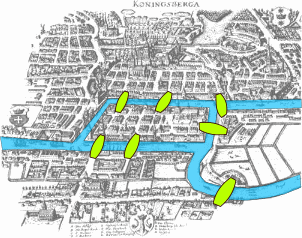
\includegraphics[width=0.4\linewidth]{Figures/Konigsberg_bridges.png} \hspace{2cm}
	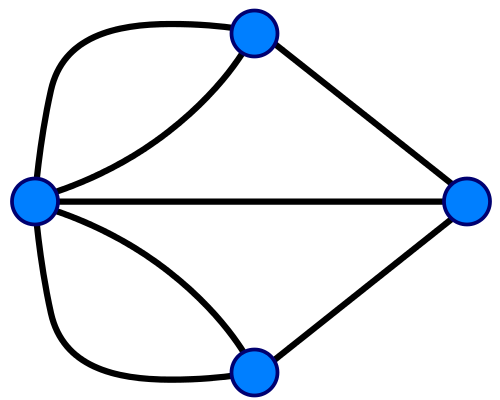
\includegraphics[width=0.4\linewidth]{Figures/Konigsberg_graph.png}
	\caption{The Kronigsber problem of seven bridges.}
	\label{fig:Krgraph}
\end{figure}

\section{Types of networks}

The seven bridges problem in Fig. \ref{fig:Krgraph} is represented with the \textbf{simple network} structure. The graph or network $G$ is defined as $G=(V, E)$, where $V$ is a set of nodes (vertices), and $E$ is a set of edges. The edge is pair of nodes $e_{ij} = (i, j), $ and $i,j\in E$. The graph structure has undirected edges meaning that edges are symmetric: $(i, j)$ implies $(j, i)$. Edges are also unweighted, meaning that all edges are equally important. The specific properties of the nodes are also neglected in this representation.\\

Sometimes it is essential to include specific properties of the system in the network representation, which can help create more realistic models. The additional properties can be added on the edge, node or network level. \\

In a \textbf{directed network}, edges have broken symmetry. The interaction from node $i$ to node $j$ does not need to have the same property as the interaction from node $j$ to node $i$. A typical example is WWW, where webpages are nodes, and hyperlinks are directed edges. In biological networks, gene regulation and neural activation can be given as directed networks. \\ %clasuet networks

%We call a directed network acyclic if it contains no cycles, i.e., for every possible i, j ∈ V , if there exists a path i → · · · → j then no path exists in the reverse direction j → · · · → i. For instance, a citation network is composed of the set of published scientific papers, and an edge (i, j) ∈ E if paper i cites paper j in its bibliography. Citation networks should be acyclic because of time: a newly published paper can only cite previously published papers, meaning each of its bibliographic links points to older papers. For a cycle to exist, some previously published paper would need to cite a non-yet-published paper, i.e., a paper in the future. (In practice, this kind of oddity does happen, as a result of preprints, and simultaneous publications.) Similarly, in food webs, predation is typically a directed and acyclic activity, with edges pointing “up” from basal species like plants or algae toward, eventually, apex predators like wolves and sharks. However, some food webs are not acyclic because species can predate themselves (cannibalism), and some pairs of species predate each other (a 2-cycle).

The frequency of interaction between nodes is emphasised if edges are associated with different scalar values; networks are \textbf{weighted}. The edges may be signed, representing activation in the biological system or trust and distrust in the social system. In general, edges can be associated with any categorical variable. If attribute describes the time when an interaction between nodes happened; network is called \textbf{temporal}. Finally, \textbf{multigraph} allows the presence of multiply edges between two nodes. For the network between cities, edges may be different driving paths between them. In neuron cells, multiply synapses are represented as distinct edges. \\

%networks with node atributes. Node atributes can be categorical data, single scalars or even vectors, representing the spatial cordinates or locations in some metric space. If nodes are cities, node atributes can include the city's population or GPS coordinates. In social networks, node atributes may include age, gender and location.

%\subsection{bipartite networks}

A \textbf{bipartite network} has two partitions, $U$ and $V$. The nodes in the same partition are not connected while links exist only between nodes of a different kind. In general, we can define k-bipartite graph. The set of nodes $V$ has $k$ distinct classes of nodes. When $k=2$ the network is bipartite.  Bipartite networks represent the membership of people or items in groups. For example, we can define the network of actors as a bipartite graph. In one partition are actors and in other movies. There are no edges between actors or movies, but the actor is connected to the film if it plays in that movie. Another example is a recommender network, such as a network of people and items they like. 

The equivalent representation of bipartite network is incidence matrix $B$. If $n$ is number of people and $g$ number of groups, this matrix is $g x n$, having elements $B_{ij}$ 1 if persoon i belongs to group j. 

Even bipartite networks give realistic representation of the system, there is often need to analyze the single type of nodes.  From a bipartite network, we can generate two projections. The first one connects nodes partition $V$ if they point to node $u$. Similarly, we can project the network on U partition, connecting $u$ nodes. The one mode projection between actors and movies onto actors is undirected network of actor collaborations. Actors are connected if they appear in the same movie. We can also create one-mode projection onto movies, where two movies are connected if they share the same actor.  

The projections are useful in some manner, but they also lose some important information, for example how many groups nodes share in common. This information can be propagated adding the weight to the edges, equal to the number of common groups.

The product $B_{ki}$ and $B_{kj}$ is 1 if $i$ and $j$ belong to the same group $k$. Thus the total number of groups to which nodes $i$ and $j$ belong is $P_{ij} = \sum_{k=1}^g B_{ki}B_{kj} = \sum_{k=1}^g B_{ik}^TB_{kj}$. The matrix $P$ is matrix of one-mode projection. The diagonal elements are non-zero, and represent the number of groups node $i$ belongs to.  To derive the weighted adjacency matrix, the diagonal elements are set to 0. The adjacency matrix of unweighted projection, each non-zero element needs to be replaced with $1$. 

The important consequence of the one-mode projection is the construction of the cliques; subgraph in which every pair of nodes is connected. Every node that is being projected is represented as a clique of size, because all pairs of its neighbours are exactly distance two away from each other. All actors in the movie will be joined in a clique in the one-mode actor projection. %ovo preformulisati

Another consequence of the one-mode projection is that one mode projection may originate from different bipartite networks. Meaning that projection is not one-to-one; no bijection. It is surjective operation, meaning hat any projected network $P$ has at least one bipartite network such that the projection of B results in P. \\ %ovo preformulisati


In \textbf{temporal networks} nodes and edges evolve over time. Many real networks are not static. Networks grow over time, edges and nodes may emerge or disappear. Also some edges may be active in regular intervals, reflecting circadian rhythms of the nodes. In citation networks, new nodes (paper) joins the network, and it creates links with cited papers. 

Let consider the temporal network with $N$ nodes, over time interval $t_{max}$. The event representation consist in viewing the temporal networks as collection of time-stamped edges. In this representation each edge $(i, j)$ is defined as$(i, j, t, \Delta t)$, where $t$ is the time of the event and $\Delta t$ its duration. In temporal network the same link can appear multiply times, and duration of the event may vary. The example of event temporal network, may be phone-calls networks, where  call between two persons $i$ and $j$ started at time $t$ and ended at $t + \Delta t$. 


A temporal network can be represented as sequence of networks $G= G(1), ... G(t_{max})$, where $t_{max}$ is number of networks. While in the event based representation time can be both discrete and continuous, in the snapshot representation time is only discrete. Temporal network is seen as structure that evolve in time and at each time stamp we are able to analyze the macroscopic properties of the system. We need to specify time windows to coarse-grain event based representation of the temporal information in the data. If we use uniformly time window of length $w$ then the events occurring in $0 \leq t < w$ enter snapshot G(1), those occurring in $w \leq t < 2w$ enter G(2) and so forth. From the snapshot representation we can not recover the original data points, and with larger time window the more information loss is present. If time window is $w=t_{max}$, there is only one snapshot, temporal data are no more available, and network is static.

%Evidence suggests that empirical networks observed in a variety of domains are far from static. It has been known since the advent of network science, and even earlier, that many networks grow in time. However, growth is not the only way in which networks evolve. Nodes and edges may emerge and disappear during the lifetime of a network. For instance, the same edge may be active just for a short period but repetitively with irregular intervals. Moreover, a rate of edge activation may depend on time. Complex dynamical patterns of networks may arise for many reasons — circadian and weekly rhythms of actors, interactions between different edges, stochasticity, finite response time of a system and so forth. These issues are at the core of the study of temporal networks, also called time/temporally varying networks/graphs, evolving graphs and evolutionary network analysis. 

%As an illustration, let us consider the networks composed of pupils and teachers in a primary school at four time points in a day, shown in Fig. 1.1. The figure indicates that the network varies over time, reflecting the daily schedule of the school. We would lose a lot of information by aggregating the four networks into one and discarding the temporal information in the original data. This includes possible correlations between edge activations, the order in which edges appear and disappear, circadian rhythms of human activity and so on. Why does temporality matter? Do we have to bother and consider this additional dimension of networks on top of already complex static networks, making things even more complicated? Does the temporality of networks significantly alter our understanding of how networked systems function? Figure 1.2 provides affirmative evidence. Figure 1.2(a) shows a temporal network composed of four individuals. The time flows along the horizontal axis. Two individuals have a conversation event when there is a vertical line. There are four conversation events. In the third one, individuals 2 and 4 talk with each other without involving individual 3. If individual 1 starts propagating news that the other three individuals have not heard of, the news can reach the entire network via conversation events.For example, individual 4 hears it from individual 2 through the path shown by the dotted arrows. However, if the news starts from individual 4, it cannot reach individual 1 within this temporal network. Although each conversation event is a symmetric event, allowing the information flow in both directions (e.g., from 1 to 2 and from 2 to 1), temporality of the network introduces asymmetry in the information flow at a network level. If we aggregate the temporal network, we obtain the static network shown in Fig. 1.2(b), which we call the aggregate network. In the aggregate network, the information on the timing of the events is discarded, and the fact that individuals 2 and 3 communicate twice in Fig. 1.2(a) is represented by an edge twice thicker than the other two edges. Aggregate networks, which are static objects, are often deceptive. In Fig. 1.2(b), individual 2 connects to everybody else and acts as a hub. A news starting from anybody can eventually reach anybody else through individual 2. However, if we unfold the temporal information, we clearly see that this conclusion is incorrect (Fig. 1.2(a)). A news starting from individual 4 cannot reach individual 1. This example is anecdotal, but it warns us of the importance of temporality in understanding network phenomena.


%In static networks, unweighted networks have originally been the major object to be studied until seminal papers emphasized the importance of weighted networks [Yook et al. (2001); Barrat et al. (2004)]. Even now, unweighted networks seem to be mainly studied. However, in temporal networks, it is a norm rather than exception that an edge is used more than once during the time course. Therefore, when we compare a given temporal network with a static counterpart, which disregards the time, the static network that we consider is often weighted. We refer to the static weighted network obtained by disregarding the time of a given temporal network, or equivalently by coarse-graining it with T w = t max , as the aggregate network. Static weighted networks are also popularly used in a snapshot representation of temporal network obtained by coarse graining. For example, G(2) and G(4) in Fig. 4.1(b) and G(1) and G(2) in Fig. 4.1(c) are weighted networks. 

%A popular variant of the snapshot representation is to use multilayer networks. Multilayer networks are a framework that considers layers of networks that are inter-related to each other [Boccaletti et al. (2014); Kivelä et al. (2014); Bianconi (2018)]. The multilayer approach to tempo- ral networks extends the snapshot representation by typically connecting the same node in the adjacent snapshots, which is called ordinal coupling, by an undirected inter-layer edge of weight w (Fig. 4.2). Because the flow of the time is unidirectional, an alternative definition is to couple layers in a biased manner such that an earlier snapshot sends inter-layer edges with a larger weight to a later snapshot than vice versa [Taylor et al. (2019a,b)].

\subsection{multiplex networks}

A network in which edges are marked by which “layer” they exist in is called a multiplex or multilayer network. These networks are used to represent a system in which there are multiple types
of interactions, and we store the connectivity of each type in a different “layer” of the multiplex
network. A temporal network is a special kind of multiplex network, where these layers form a
temporal (ordered) sequence. Crucially, there can dynamics on each vertex that govern which layer
some kind of interaction occurs on, so multiplex networks are not merely a special kind of graph
in which edges are annotated by different colors or layer numbers.

Spatial networks are a special kind of node-annotated network, in which the annotations repre-
sent the node’s location in some d-dimensional space. This graph property is most common in
transportation networks, e.g., as road and city networks, airport transportation networks, oil and
gas distribution networks, shipping networks, etc., but can also appear in social networks. Planar
graphs are a special case of spatial networks, in which the nodes are embedded on a 2-dimensional
surface and edges do not cross.

Hypergraphs are another type of network, in which edges denote the interaction of more than two
vertices, e.g, E in V × V × V . Scientific collaboration graphs can be represented as a hypergraph,
in which each “edge” is the set of coauthors on a scientific article. However, collaboration networks
are more commonly represented as bipartite graphs, in which scientists and papers form two sets
of vertices, and scientist-nodes are connected to all the paper-nodes on which they are authors.


